\documentclass{beamer}

\mode<presentation>
{
  \usetheme{CambridgeUS}      % or try Darmstadt, Madrid, ...
  \usecolortheme{default} % or try albatross, beaver, crane, ...
  \usefonttheme{default}  % or try serif, structurebold, ...
  \setbeamertemplate{navigation symbols}{}
  \setbeamertemplate{caption}[numbered]
} 

\usepackage[english]{babel}
\usepackage[utf8x]{inputenc}
\usepackage{listings}
\usepackage[ampersand]{easylist}



\definecolor{KTI_green}{RGB}{150, 189, 13}
\definecolor{TU_red}{RGB}{255, 55, 81}
\definecolor{faint_gray}{RGB}{180, 180, 180}

\definecolor{syntax_green}{rgb}{0,0.6,0}
\definecolor{syntax_gray}{rgb}{0.9, 0.9, 0.9}
\definecolor{syntax_mauve}{rgb}{0.58,0,0.82}

\lstset{ 
  backgroundcolor=\color{syntax_gray},  % choose the background color
  basicstyle=\scriptsize\ttfamily,        		% size of fonts used for the code
  breaklines=false,                		% automatic line breaking only at whitespace
  captionpos=b,                    		% sets the caption-position to bottom
  commentstyle=\color{syntax_green},    % comment style
  escapeinside={\%*}{*)},          		% if you want to add LaTeX within your code
  keywordstyle=\color{blue},       		% keyword style
  stringstyle=\color{syntax_mauve},     % string literal style
  columns=fullflexible,
  frame=single,
  framesep=0.5cm,
  framexleftmargin=0.5cm,
  xleftmargin=0.5cm,
  framexrightmargin=0.5cm,
  xrightmargin=0.5cm,
  frame=tb,                 
    numbers=left,                    
    numbersep=15pt,  
  }
  
  
\newcommand{\logopython}{\raggedleft 
\includegraphics[height=0.5cm]{logo_python}\hspace{0.1cm}\\\raggedright}
\newcommand{\logopythonbottom}{\raggedleft\vspace{-0.8cm}
\includegraphics[height=0.5cm]{logo_python}\hspace*{0.05cm}\\\raggedright}

\title[BSP13 - Simulation von $\pi$]{Simulation von $\pi$}
\author{Dickbauer Y., Moser P., Perner M.}
\institute{PS Computergestützte Modellierung, WS 2016/17}
%\date{Date of Presentation}

\begin{document}

\begin{frame}
  \titlepage
\end{frame}

% Uncomment these lines for an automatically generated outline.
\begin{frame}{Outline}
  \tableofcontents
\end{frame}

\section{Aufgabenstellung}
\begin{frame}{Aufgabenstellung}
Berechnen Sie näherungsweise mittels Simulation die Zahl $\pi$ (3.14159) (Hinweis: Einheits(viertel)kreis)
\begin{itemize}
  \item Eingabe: Anzahl an Punkten
  \item Output: Pi
\end{itemize}

\end{frame}

\begin{frame}{Grafische Darstellung anhand des Einheitskreises}
  \begin{columns}[onlytextwidth]
    \begin{column}{0.7\textwidth}
	\centering
  	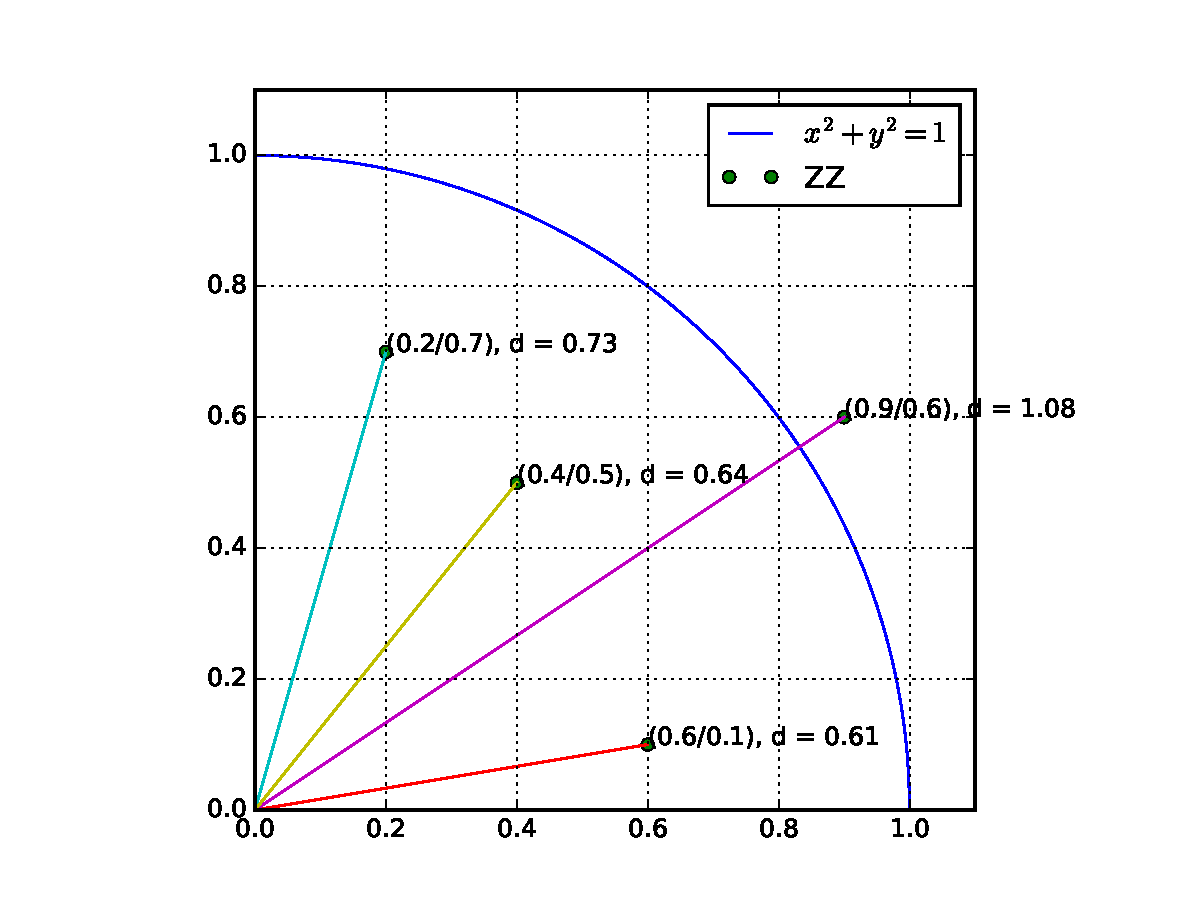
\includegraphics[scale=0.5]{BSP13_plot_monte_carlo_simulation.pdf}
  \end{column}

    \begin{column}{0.2\textwidth}
      \begin{block}{Fläche des Viertelkreises}
        $\frac{1}{4} * A_{Kreis}$\\
        = \\
        $\frac{1}{4}* 1^2 * \pi$      
      \end{block}
            \begin{block}{WSK, dass ZZ innerhalb}
	        $p = \frac{\pi}{4}$      
      \end{block}
      \end{column}
      \end{columns}
\end{frame} 

\section{Flow Chart}
\begin{frame}{Flow Chart}
	\centering
  	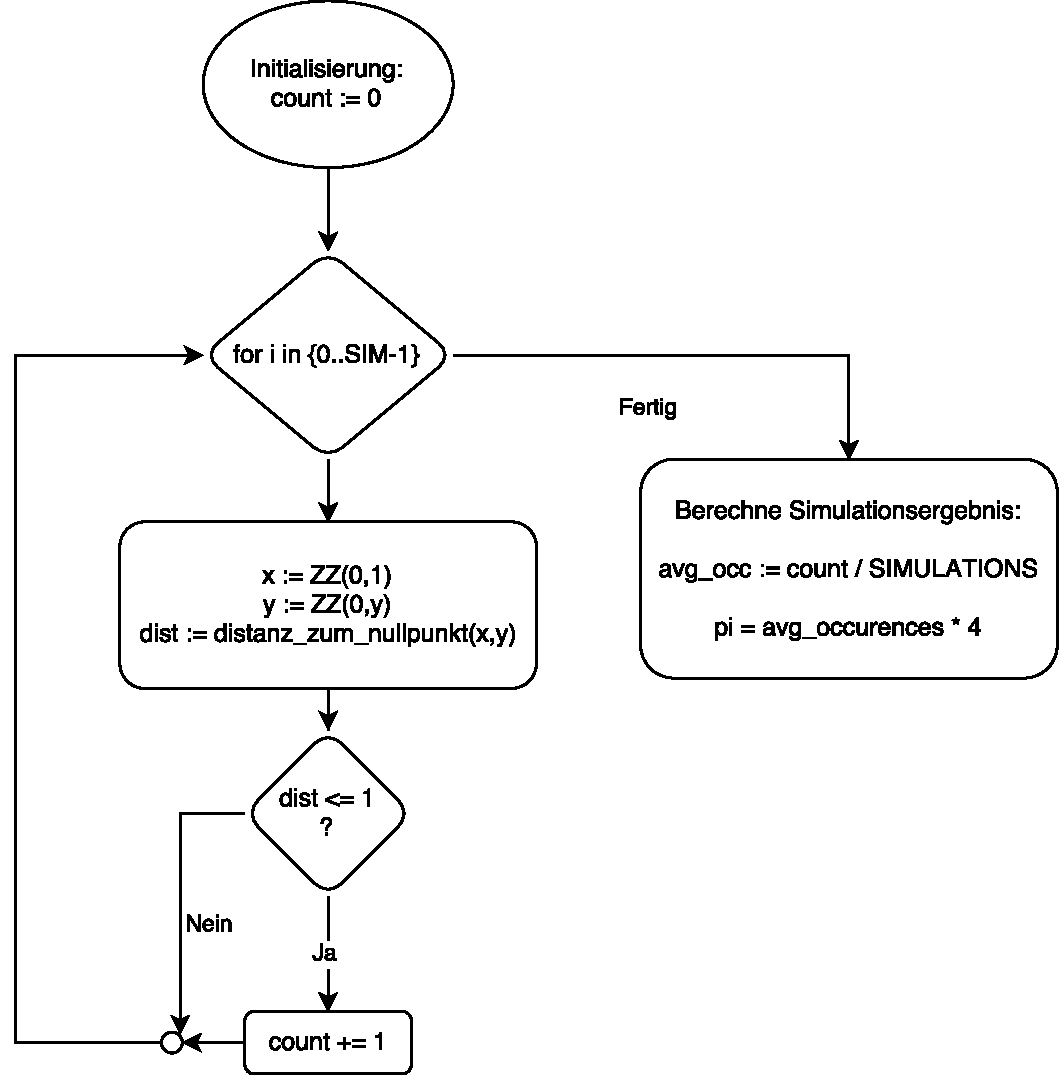
\includegraphics[scale=0.4]{BSP13_Flow_Chart.pdf}
\end{frame}

\section{Programmcode}
\subsection{Main Funktion}
\begin{frame}[fragile]{Main Funktion - Programmeinstieg}
  \begin{lstlisting}[language=python]
def main():
    # user input:
    simulations = user_input((
        ('Number of simulations', int, 10000), ),DEBUG)[0]
        
    count = 0 # how often did we shoot in the unit circle
    
    for i in range(simulations):
        # create two randoms representing cords in a [1,1] rectangle
        x = random_number_from_interval(0,1)
        y = random_number_from_interval(0,1)
        # check wheter these cords are lying within or beyond the unit circle
        if euclidean_distance((0, 0), (x, y)) <= 1:
            count += 1
        
    # avg_occurrences p should be pi/4 / 1 --> 4 * avg = pi
    avg_occurrences = count/simulations
    pi = avg_occurrences * 4
    print('Pi is simulated:', pi)
    print('Difference:     {:+.5f} %'.format((pi/REFERENCE_PI - 1) * 100))
\end{lstlisting}
\logopythonbottom
\end{frame}

\subsection{Verwendete Funktionen}
 \begin{frame}[fragile]{Funktion euclidean\_distance(p1, p2)}
  \begin{itemize}
    \item Diese Funktion verlangt zwei Punkte (x1, y1) (x2, y2) als Eingabeparameter
    \item Gibt die eukliedsche Distanz zurück
  \end{itemize}
  \begin{lstlisting}[language=python]
def euclidean_distance(point_1, point_2):
    """
        Calculates the euclidean distance between two points
        
        point_1: a tuple of (x,y) values
        point_2: a tuple of (x,y) values
    """
    delta_x = point_2[0] - point_1[0]
    delta_y = point_2[1] - point_1[1]
    return (delta_x ** 2 + delta_y ** 2) ** 0.5
\end{lstlisting}
\logopythonbottom
\end{frame}	
%\begin{frame}[fragile]{Funktion random\_number\_from\_interval(..)}
  \begin{itemize}
    \item Diese Funktion verlangt zwei Eingabeparameter \textit{lower} und \textit{upper}
    \item Gibt eine (pseudo)Zufallszahl (\textit{float}) im Intervall  [\textit{lower}, \textit{upper}) zurück 
    \item \textit{random.random()} ist eine Funktion der Python Standardbibliothek, welche ein Zufallszahl (\textit{float}) im Intervall [\textit{lower}, \textit{upper}) zurück gibt
    \item Mersenne Twister Methode wird als Generator der ZZ verwendet\footnote[frame] {\scriptsize\url{https://docs.python.org/3.5/library/random.html}} \footnote[frame] {\scriptsize\url{https://en.wikipedia.org/wiki/Mersenne_Twister}}
  \end{itemize}
  \begin{lstlisting}[language=python]
def random_number_from_interval(lower, upper):
    val = random.random()
    return lower + (upper -lower) * val
\end{lstlisting}
\logopythonbottom
\end{frame}	
%\begin{frame}[fragile]{Funktion user\_input(input\_vars, [use\_defaults])}
  \begin{itemize}
  	\item Diese Funktion verlang vom User die geforderten Eingabeparameter und gibt diese als von der Programmiererin gewünschten Datentyp wieder zurück
    \item Funktion verlangt als ersten Eingabeparameter die Liste \textit{input\_vars}
    \item Falls \textit{use\_defaults == True} wird der User nicht nach Eingabe gefragt (Dient zum Testen)
    \item Diese Liste besteht wiederrum aus Listen mit je Länge = 3:
    \begin{itemize}
    	\item 0: Text, welcher dem User ausgegeben wird
    	\item 1: Datentyp (int/float/str)
    	\item 2: Default value: Dieser Wert wird zurueckgegeben, falls \textit{use\_defaults == True}
    \end{itemize}
  \end{itemize}
  \begin{lstlisting}[language=python]
x, y = user_input((
    ('Geben Sie einen X Wert ein', int, 10),
    ('Geben Sie einen Y Wert ein', int,  5), False):
  \end{lstlisting}
  \logopythonbottom
\end{frame}	

\section{Beispiel}
\begin{frame}[fragile]{Beispiel anhand fixer Zufallszahlen}
\begin{itemize}
\item Annahme der Zufallszahlen wie folgt:
\end{itemize}
\begin{center}
  \begin{tabular}{c|c|c|c|c}
  \hline 
  iteration & 0 & 1 & 2 & 3\\ 
  \hline 
  x      & 0.6 & 0.2 & 0.9 & 0.4 \\ 
  y      & 0.1 & 0.7 & 0.6 & 0.5 \\
  \hline 
  dist   & 0.61 & 0.73 & 1.08 & 0.64 \\
  Im Kreis? & 1 & 1 & 0 & 1 
  \end{tabular} 
\end{center}
\begin{easylist}
\ListProperties(Hide=100, Hang=true, Progressive=3ex, Style*= ,
Style2*=$\bullet$ ,Style3*=$\circ$ ,Style4*=\tiny$\blacksquare$ )
& count = 3
& iterations = 4
& avg\_occ = $\frac{3}{4}$
& pi\_sim = $4 \frac{3}{4} = 3.0 $
& abweichung: -4.5%
\end{easylist}
\end{frame}

\begin{frame}{Grafische Darstellung des Beispiels}
	\centering
  	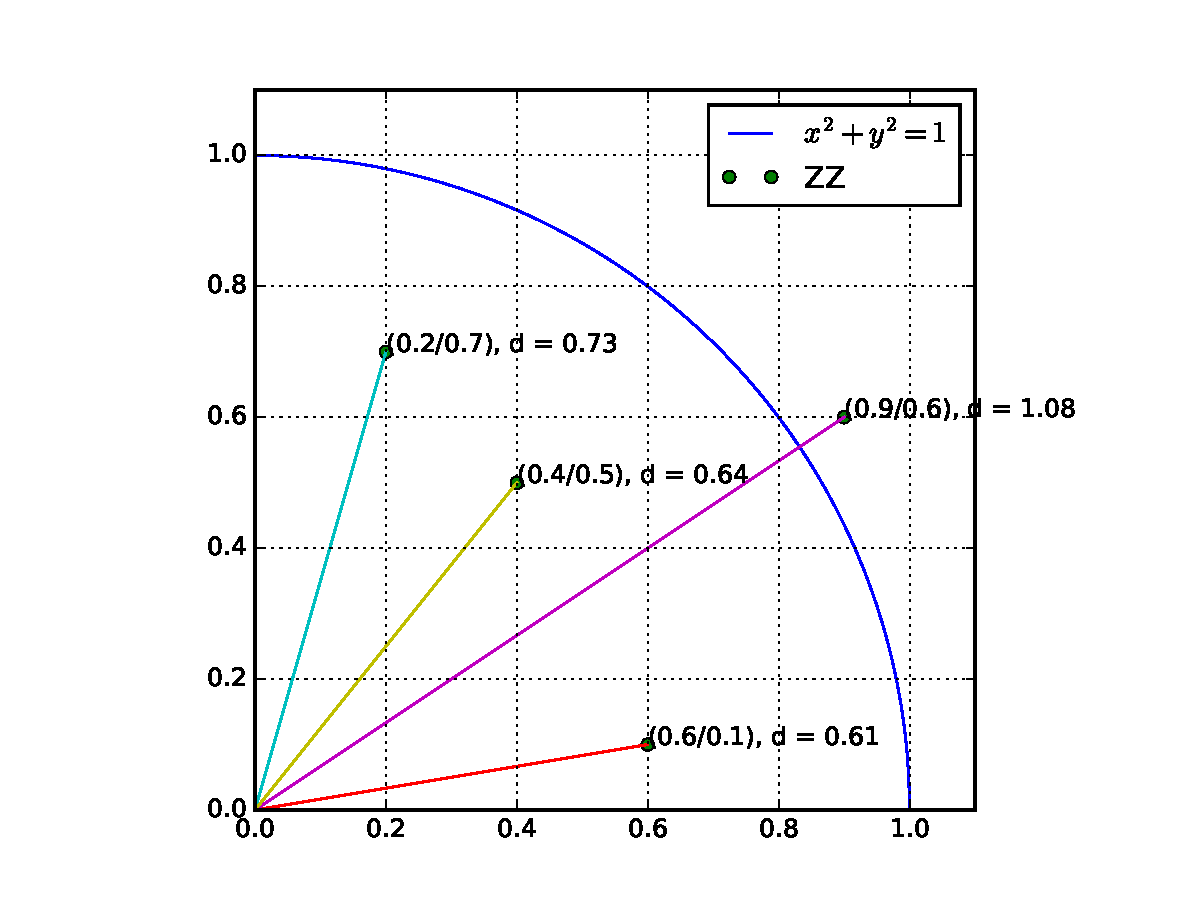
\includegraphics[scale=0.5]{BSP13_plot_monte_carlo_simulation.pdf}
\end{frame} 

\begin{frame}[fragile]{Anhang: Modifikation des Source Codes um Demo Beispiel zu erhalten}
  \begin{lstlisting}[language=python]
  #  Fuege folgenden Code vor der main() Funktion ein:
ZZ = [0.6, 0.1,   0.2, 0.7,  0.9, 0.6,   0.4, 0.5] * 1000
i = -1
def random_number_from_interval(x,y):
    global i
    i += 1
    return ZZ[i]
  \end{lstlisting}
\logopythonbottom
\end{frame}
\end{document}
